\chapter{Fundamentos teóricos}

El modelado y renderizado en 3D es posible gracias a una serie de técnicas
matemáticas y computacionales que permiten representar, manipular y visualizar
geometría en entornos virtuales. Copper se apoya principalmente en el modelado
mediante funciones de distancia con signo (SDF), el renderizado por ray
marching y el uso del estándar gráfico WebGPU. Este capítulo describe en
profundidad cada uno de estos fundamentos.

\section{Modelado tridimensional: Paradigmas y fundamentos}

El modelado tridimensional tradicional utiliza mallas poligonales, donde los
objetos se representan mediante vértices, aristas y caras conectadas entre sí.
Este método, empleado en la mayoría de herramientas profesionales
(\textit{Blender, Maya, 3ds Max}), permite una gran flexibilidad, pero implica
gestionar topología y almacenar grandes cantidades de datos, lo que complica la
edición y la generación procedural.

Como alternativa, existen métodos de representación implícita, siendo los
campos de distancia con signo (\textit{Signed Distance Fields, SDF}) los más
destacados. Una SDF es una función $f(\vec{x})$ que, para cada punto $\vec{x}$
del espacio, devuelve la distancia mínima a la superficie del objeto. El signo
indica si el punto está en el interior (negativo), sobre la superficie (cero) o
en el exterior (positivo). Este enfoque permite describir objetos mediante
expresiones matemáticas, simplificando la combinación y manipulación de
geometría compleja.

\subsection{Ventajas de las SDF frente al modelado poligonal}

\begin{itemize}
    \item \textbf{Compacidad}: Las SDF están definidas por fórmulas matemáticas, no por listas de vértices, lo que reduce el espacio necesario para describir objetos.
    \item \textbf{Facilidad de combinación}: Pueden combinarse mediante operadores matemáticos (unión, intersección, resta) de forma eficiente.
    \item \textbf{Transformaciones geométricas}: Admiten fácilmente traslaciones, rotaciones y escalados aplicando transformaciones sobre la función.
    \item \textbf{Cálculo de normales}: La normal en un punto de la superficie se obtiene como el gradiente de la función de distancia.
    \item \textbf{Flexibilidad}: Permiten crear transiciones suaves entre objetos mediante operadores suavizados.
\end{itemize}

\section{Funciones de distancia con signo (SDF)}

Las SDF asignan a cada punto del espacio la distancia mínima a una superficie
implícita. Formalmente, para una función $f(\vec{x})$, la superficie se define
como el conjunto de puntos donde $f(\vec{x}) = 0$. Las SDF permiten describir
primitivas básicas como:

\begin{itemize}
    \item \textbf{Esfera}: $f_{esfera}(\vec{x}) = ||\vec{x} - \vec{c}|| - r$, donde $\vec{c}$ es el centro y $r$ el radio.
    \item \textbf{Caja}: $f_{caja}(\vec{x}) = ||\max(|\vec{x} - \vec{c}| - \vec{s}, 0)|| + \min(\max(d_x, \max(d_y, d_z)), 0)$, donde $\vec{s}$ es el tamaño.
\end{itemize}

Las SDF pueden combinarse empleando operadores booleanos y suaves:

\begin{itemize}
    \item \textbf{Unión}: $f_{union}(a, b) = \min(a, b)$
    \item \textbf{Intersección}: $f_{inter}(a, b) = \max(a, b)$
    \item \textbf{Resta}: $f_{resta}(a, b) = \max(a, -b)$
    \item \textbf{Unión suave}: Interpolación entre distancias y colores para crear transiciones continuas.
\end{itemize}

\subsection{Propiedades y aplicaciones}

Las SDF permiten:

\begin{itemize}
    \item Evaluar la función en cualquier punto del espacio para detectar colisiones,
          calcular iluminación o generar geometría procedural.
    \item Calcular la normal en un punto como el gradiente $\nabla f(\vec{x})$.
    \item Construir geometría fractal y orgánica mediante funciones recursivas o
          combinaciones arbitrarias.
\end{itemize}

Se emplean en renderizado, simulación física, generación de terrenos y efectos
visuales avanzados.

\section{Ray Marching}

El \textit{ray marching} es una técnica de renderizado que, utilizando la SDF,
avanza iterativamente un rayo en el espacio hasta aproximar la intersección con
una superficie implícita.

El algoritmo sigue estos pasos:

\begin{enumerate}
    \item Lanzar un rayo desde la cámara en una dirección determinada.
    \item Evaluar la SDF en la posición actual para obtener la distancia mínima a la
          superficie más cercana.
    \item Avanzar el punto a lo largo del rayo una distancia igual al valor obtenido.
    \item Repetir hasta que la distancia sea menor que un umbral (colisión con la
          superficie) o se alcance un límite de pasos o distancia máxima.
\end{enumerate}

\subsection{Comparación con Ray Tracing}

\begin{itemize}
    \item \textbf{Ray tracing}: Calcula la intersección exacta con primitivas geométricas.
    \item \textbf{Ray marching}: Utiliza la distancia local para aproximar superficies implícitas y fractales.
\end{itemize}

Ray marching facilita la incorporación de sombras suaves, reflexión y
refracción, y la renderización eficiente de geometría compleja.

\subsection{Sphere Tracing}

La técnica de \textbf{sphere tracing} es una variante eficiente del ray
marching, utilizada específicamente para el renderizado de superficies
implícitas definidas por funciones de distancia con signo (SDF). Su principal
ventaja respecto a los métodos tradicionales de ray casting es que utiliza la
propia SDF para calcular el avance óptimo en cada paso del rayo, evitando
colisiones innecesarias y acelerando la detección de intersecciones.

El algoritmo se basa en la siguiente idea: desde el origen del rayo, en cada
iteración se evalúa la SDF en la posición actual para obtener la distancia
mínima a cualquier superficie. Este valor se interpreta como el radio de una
esfera libre de obstáculos centrada en el punto actual. Así, se puede avanzar
el rayo exactamente esa distancia sin riesgo de atravesar ninguna superficie.
El proceso se repite hasta que la distancia es menor que un umbral prefijado
(lo que indica que se ha alcanzado la superficie) o hasta que se supera una
distancia máxima o número de pasos.

Sphere tracing es especialmente útil en escenas donde las funciones de
distancia son suaves y bien definidas, y permite renderizar geometría compleja
con costes computacionales bajos. Sin embargo, puede resultar menos eficiente
en casos de superficies muy delgadas o SDFs poco continuas, donde el avance
óptimo se reduce drásticamente.

La Figura~\ref{fig:sphere-tracing} ilustra el funcionamiento del algoritmo:
cada círculo representa el rango libre de obstáculos desde la posición actual
del rayo, determinado por la evaluación de la SDF. El rayo avanza saltando de
esfera en esfera hasta que la distancia mínima indica una colisión con la
superficie.

\begin{figure}[H]
    \centering
    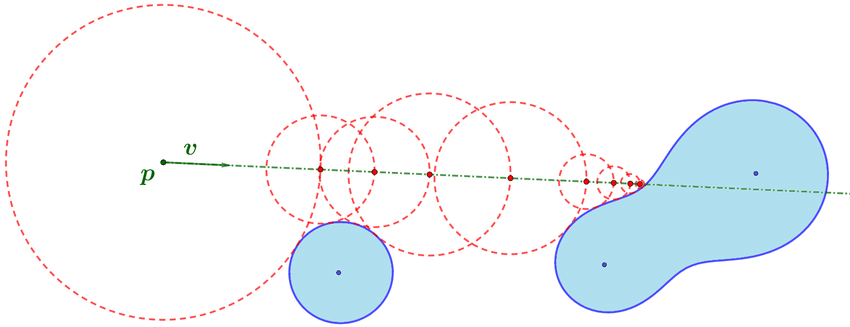
\includegraphics[width=0.6\textwidth]{sphere_tracing.png}
    \caption{Representación visual del algoritmo de sphere tracing.}
    \label{fig:sphere-tracing}
\end{figure}

\section{WebGPU: Acceso moderno a la GPU}

\textbf{WebGPU} es un estándar gráfico de nueva generación que proporciona acceso eficiente y multiplataforma a la GPU, tanto en navegadores como en aplicaciones nativas. Sus principales características incluyen:

\begin{itemize}
    \item Multiplataforma: Compatible con Windows, Linux, Mac y navegadores recientes.
    \item Eficiencia: Modelo de programación cercano al hardware, acceso directo a
          buffers y pipelines.
    \item Shaders en WGSL: Permite la programación de efectos personalizados y
          operaciones matemáticas avanzadas.
\end{itemize}

WebGPU ofrece ventajas frente a OpenGL y DirectX en control de recursos,
computación general y portabilidad.

\section{Shaders y lenguaje WGSL}

Los \textbf{shaders} son programas que ejecutan operaciones matemáticas en la
GPU para transformar vértices, calcular colores y simular efectos visuales.

WGSL (\textit{WebGPU Shading Language}) es el lenguaje nativo de WebGPU,
diseñado para expresar funciones de distancia, operadores booleanos, cálculos
de iluminación y efectos visuales de forma eficiente.

\begin{itemize}
    \item \textbf{Vertex shaders}: Transforman posiciones y atributos de vértices.
    \item \textbf{Fragment shaders}: Calculan el color final de cada píxel, aplicando modelos de iluminación como Blinn-Phong, efectos de sombras y combinaciones de SDF.
\end{itemize}

WGSL permite aprovechar la arquitectura de la GPU para realizar renderizado en
tiempo real.

\section{Herramientas auxiliares}

El desarrollo de aplicaciones gráficas requiere gestionar ventanas, entrada de
usuario y la interfaz gráfica:

\begin{itemize}
    \item \textbf{GLFW}: Biblioteca multiplataforma para la gestión de ventanas y eventos.
    \item \textbf{ImGui}: Sistema de interfaz gráfica inmediata para la manipulación interactiva de primitivas y parámetros de escena.
    \item \textbf{GLM}: Biblioteca matemática para operaciones con vectores y matrices.
    \item \textbf{CMake}: Herramienta de compilación y gestión de dependencias.
\end{itemize}

Estas herramientas proporcionan la infraestructura básica para la interacción y
visualización dentro del entorno de Copper.
